\documentclass[a4paper, 12pt]{article}
% A4纸张,article类型
\usepackage[UTF8]{ctex}
%以此支持中文
\usepackage{graphicx}
%以此插入图片
\usepackage{url}
%支持使用 \url命令
\usepackage{float}
\usepackage{xcolor}
\usepackage{hyperref} % 加载hyperref宏包 
\usepackage{listings}  % 代码高亮包
\usepackage{amsmath}
\usepackage{verbatim}

\begin{document}
  \title{第二节课实验报告}
  \author{王书一 \\ 23020007119}
  \date{August 30, 2024}
  \maketitle

 \pagenumbering{arabic}
 \tableofcontents
 \newpage
 \pagenumbering{arabic}
 %目录

  
  \section{实验目的}
   本实验旨在掌握Shell工具与脚本的基本操作,熟悉常用命令及其组合使用方式,学会通过正则表达式进行高级数据处理,了解如何通过Shell工具进行数据处理和文件处理。
  
\section{实验环境}
\begin{itemize}
    \item 操作系统:Ubuntu 20.04
    \item 使用终端:bash
    \item 编辑器:vim
    \item 工具:grep、sed、awk、sort、echo、cut
\end{itemize}

\section{shell工具和脚本}

\subsection{基本shell命令}

\textbf{ls} - 列出目录中的文件和文件夹:
\begin{itemize}
    \item \texttt{ls}           列出当前目录的文件和文件夹
    \item \texttt{ls -l}        以长格式列出文件,显示更多信息
    \item \texttt{ls -a}        显示所有文件,包括隐藏文件
    \item \texttt{ls -lh}      以人类可读的格式显示文件大小
\end{itemize}

\begin{figure}[H]
  \centering
    \includegraphics[width=0.9\linewidth]{18.png}
  \caption{ls命令}
   \end{figure}
   
\textbf{cd} - 更改当前工作目录:
\begin{itemize}
    \item \texttt{cd /path/to/directory}  % 切换到指定目录
    \item \texttt{cd \textasciitilde}      % 切换到用户的主目录
    \item \texttt{cd ..}                  % 返回上一级目录
\end{itemize}


 

\subsection{shell工具}  
\begin{lstlisting}
top           实时显示 CPU、内存、进程等系统信息
\end{lstlisting}
\begin{figure}[H]
  \centering
    \includegraphics[width=0.9\linewidth]{19.png}
  \caption{top命令}
   \end{figure}

\subsection{shell工具应用}  
使用 ls 命令进行如下操作:

所有文件(包括隐藏文件)
文件打印以人类可以理解的格式输出 (例如,使用 454M 而不是 454279954)
文件以最近访问顺序排序
以彩色文本显示输出结果

\begin{lstlisting}
ls -lAh --time=atime --color=auto
\end{lstlisting}
具体说明:

-l:以长格式列出文件信息。
-A:显示所有文件(包括隐藏文件),但不显示 . 和 ..。
-h:以人类可读的格式显示文件大小(如 1.1M 而不是字节数)。
--time=atime:按照最近的访问时间排序。
--color=auto:为不同的文件类型显示不同的颜色。
\begin{figure}[H]
  \centering
    \includegraphics[width=0.9\linewidth]{20.png}
  \caption{ls命令应用}
   \end{figure}

  \subsection{marco和polo函数}  
  编写两个 bash 函数 marco 和 polo 执行下面的操作。 每当你执行 marco 时,当前的工作目录应当以某种形式保存,当执行 polo 时,无论现在处在什么目录下,都应当 cd 回到当时执行 marco 的目录。
\begin{lstlisting}
下面是 marco.sh 文件的内容:
#!/bin/bash
# marco 函数:保存当前工作目录到环境变量
marco() {
    export MARCO_DIR=$(pwd)
    echo "Directory saved: $MARCO_DIR"
}
# polo 函数:切换到上次保存的目录
polo() {
    if [ -z "$MARCO_DIR" ]; then
        echo "No directory saved. Run 'marco' first."
    else
        cd "$MARCO_DIR" || echo "Failed to change directory to $MARCO_DIR"
    fi
}
\end{lstlisting}
\begin{figure}[H]
  \centering
    \includegraphics[width=0.9\linewidth]{21.png}
  \caption{marco和polo的实现}
   \end{figure}

\subsection{判定用户输入的字符类型脚本}  
\begin{lstlisting}
#!/bin/bash
read -p "请输入一个字符,并按Enter确认:" KEY
case "$KEY" in
	[a-z]|[A-Z])
	echo "您输入的是字母"
	;;
	
	[0-9])
	echo "您输入的是数字"
	;;
	
	*)
	echo "您输入的是其他字符"
	;;
esac
\end{lstlisting}
输入 a 或 Z,它将输出:
您输入的是字母
输入 5,它将输出:
您输入的是数字
输入 @,它将输出:
您输入的是其他字符
\begin{figure}[H]
  \centering
    \includegraphics[width=0.9\linewidth]{22.png}
  \caption{if-case脚本}
   \end{figure}

\subsection{记录命令出错的脚本}  
假设您有一个命令,它很少出错。因此为了在出错时能够对其进行调试,需要花费大量的时间重现错误并捕获输出。 编写一段 bash 脚本,运行如下的脚本直到它出错,将它的标准输出和标准错误流记录到文件,并在最后输出所有内容。 加分项:报告脚本在失败前共运行了多少次。
\begin{lstlisting}
 #!/usr/bin/env bash

 n=$(( RANDOM % 100 ))

 if [[ n -eq 42 ]]; then
    echo "Something went wrong"
    >&2 echo "The error was using magic numbers"
    exit 1
 fi

 echo "Everything went according to plan"
\end{lstlisting}
 编写一个 bash 脚本,将给定命令不断运行,直到发生错误,同时将标准输出和标准错误都记录到文件中。脚本还会在结束时输出错误发生前运行的次数。
 以下是脚本的内容:
\begin{lstlisting}
#!/usr/bin/env bash

logfile="script_output.log"
count=0

# 清空 log 文件
> "$logfile"

while true; do
  ((count++))
  
  # 运行命令并捕获标准输出和标准错误
  output=$(./your_script.sh 2>&1)
  
  # 将输出追加到日志文件
  echo "Run #$count" >> "$logfile"
  echo "$output" >> "$logfile"
  echo "-------------------------" >> "$logfile"
  
  # 检查命令是否失败
  if [[ $? -ne 0 ]]; then
    echo "Script failed after $count runs"
    echo "Full log is available in $logfile"
    cat "$logfile"
    exit 1
  fi
done
解释:
logfile="script_output.log":定义日志文件名。
> "$logfile":清空日志文件。
while true; do ... done:持续运行给定命令直到出错。
./your_script.sh 2>&1:运行 your_script.sh,将标准输出和标准错误合并。
if [[ $? -ne 0 ]]; then:检测命令是否返回错误状态码。
echo "Run #$count":将每次运行的计数写入日志文件。
cat "$logfile":在出错时显示所有日志。
这个脚本会不断运行 your_script.sh,直到遇到错误,
并在最后输出总运行次数及完整日志。
输出结果
Script failed after 7 runs
Full log is available in script_output.log
\end{lstlisting}

\begin{figure}[H]
  \centering
    \includegraphics[width=0.9\linewidth]{23.png}
  \caption{运行结果}
   \end{figure}
\begin{figure}[H]
  \centering
    \includegraphics[width=0.9\linewidth]{24.png}
  \caption{运行结果}
   \end{figure}
   输出结果:
Script failed after 7 runs
Full log is available in script\_output.log

\subsection{shell计算脚本}  
\begin{lstlisting}
#!/bin/bash
read -p "请输入第一个数字: " NUM1
read -p "请输入第二个数字: " NUM2
SUM=$((NUM1 + NUM2))
echo "它们的和是: $SUM"
\end{lstlisting}
\begin{figure}[H]
  \centering
    \includegraphics[width=0.9\linewidth]{25.png}
  \caption{计算结果}
   \end{figure}

  \subsection{shell查找文件脚本}  
\begin{lstlisting}
#!/bin/bash
read -p "请输入要检查的文件名: " FILENAME
if [ -e "$FILENAME" ]; then
    echo "文件 '$FILENAME' 存在。"
else
    echo "文件 '$FILENAME' 不存在。"
fi
\end{lstlisting}

\begin{figure}[H]
  \centering
    \includegraphics[width=0.9\linewidth]{26.png}
  \caption{查找文件结果}
   \end{figure}

\subsection{统计和、最小}  
\begin{lstlisting}
#!/bin/bash  
COUNT=1  
SUM=0  
MIN=0  
MAX=100  
while [ $COUNT -le 5 ]; do  
    read -p "请输入1-10个整数:" INT      
    if [[ ! $INT =~ ^[0-9]+$ ]]; then  
        echo "输入必须是整数!"  
        exit 1  
    elif [[ $INT -gt 100 ]]; then  
        echo "输入必须是100以内!"  
        exit 1  
    fi  
    SUM=$(($SUM+$INT))  
    [ $MIN -lt $INT ] && MIN=$INT  
    [ $MAX -gt $INT ] && MAX=$INT  
    let COUNT++  
    done  
echo "SUM: $SUM"  
echo "MIN: $MIN"   
\end{lstlisting}
\begin{figure}[H]
  \centering
    \includegraphics[width=0.9\linewidth]{28.png}
  \caption{运行结果}
   \end{figure}
   
\section{编辑器(vim)}
\subsection{vim的使用}  
\begin{lstlisting}
1. 使用 vim 编辑脚本文件:
假设脚本名为 your_script.sh,可以使用以下命令在 vim 中打开并编辑它:
vim your_script.sh
在 vim 中,可以进行以下操作:
按 i 进入插入模式并编辑脚本内容。
编辑完成后,按 Esc 退出插入模式。
输入 :wq 保存文件并退出 vim。
2. 使用 vim 查看日志文件:
想检查运行脚本后的日志输出时,可以使用 vim 打开日志文件,例如 script_output.log:
vim script_output.log
在 vim 中,你可以使用以下快捷键浏览日志内容:
上下箭头或 j/k:向下或向上滚动。
G:跳到文件末尾。
gg:跳到文件开头。
输入 :q 退出 vim。
\end{lstlisting}
\begin{figure}[H]
  \centering
    \includegraphics[width=0.9\linewidth]{27.png}
  \caption{使用vim进行编辑}
   \end{figure}

\section{数据整理}
\begin{itemize}
    \item 数据过滤:使用  grep 来筛选指定条件的日志条目
    \item 数据格式化:使用 sed 和 awk 来替换或格式化日志条目
    \item 数据排序:使用 sort 对过滤后的数据进行排序
\end{itemize}

\subsection{使用 grep 进行数据筛选}
我们将首先从日志文件中筛选包含关键字“ERROR”的行。为了便于测试,假设我们有一个名为 `log.txt` 的日志文件,其内容如下:

\begin{lstlisting}
INFO 2024-09-06 Connection established.
ERROR 2024-09-06 Connection lost.
INFO 2024-09-06 Attempting to reconnect.
ERROR 2024-09-06 Reconnection failed.
INFO 2024-09-06 Connection re-established.
\end{lstlisting}

要筛选出所有的错误条目,使用以下命令:

\begin{lstlisting}[language=bash]
grep ERROR log.txt
\end{lstlisting}

执行结果如下:

\begin{lstlisting}
ERROR 2024-09-06 Connection lost.
ERROR 2024-09-06 Reconnection failed.
\end{lstlisting}

\begin{figure}[H]
  \centering
    
\includegraphics[width=0.7\linewidth]{1.png}
  \caption{log.txt}
   \end{figure}
   
\begin{figure}[H]
  \centering
    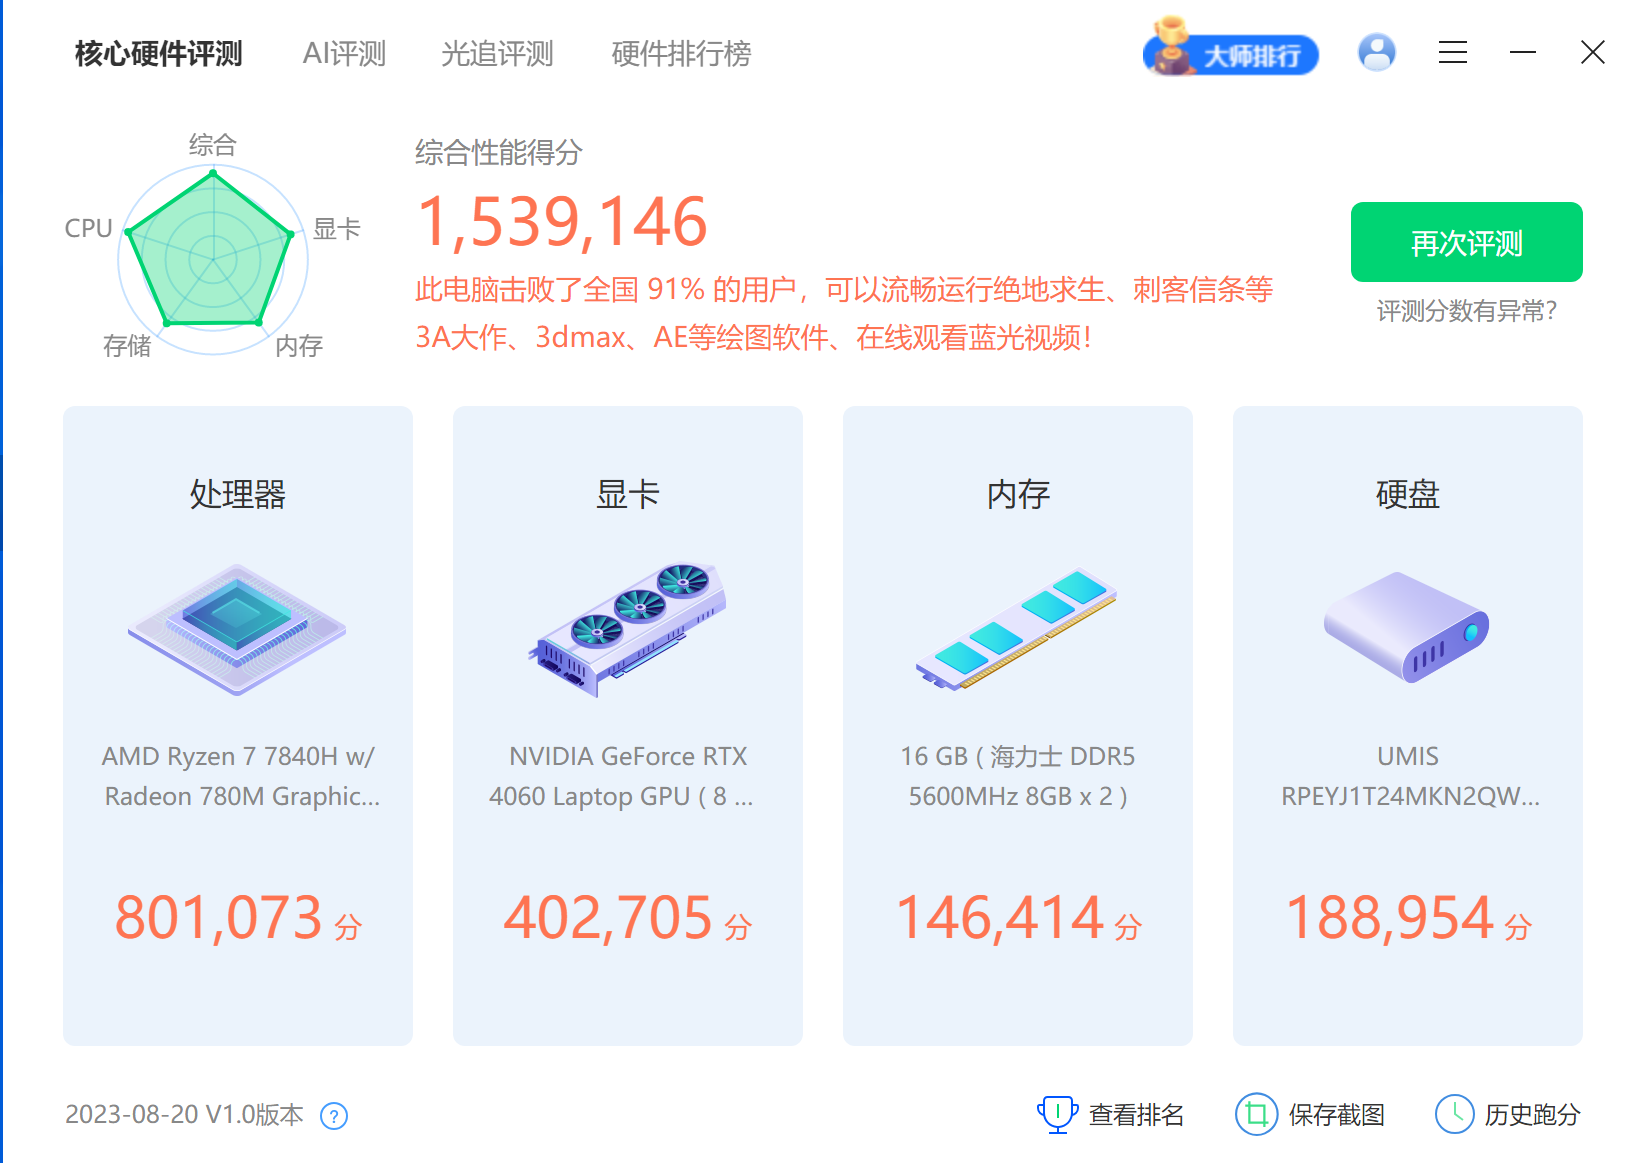
\includegraphics[width=0.7\linewidth]{2.png}
  \caption{grep进行数据筛选}
   \end{figure}

\subsection{使用 sed 进行数据替换}
假设我们想要将所有的“ERROR”关键字替换为“WARNING”,可以使用 `sed` 命令:

\begin{lstlisting}[language=bash]
sed 's/ERROR/WARNING/g' log.txt
\end{lstlisting}

输出结果将是:

\begin{lstlisting}
INFO 2024-09-06 Connection established.
WARNING 2024-09-06 Connection lost.
INFO 2024-09-06 Attempting to reconnect.
WARNING 2024-09-06 Reconnection failed.
INFO 2024-09-06 Connection re-established.
\end{lstlisting}

\begin{figure}[H]
  \centering
    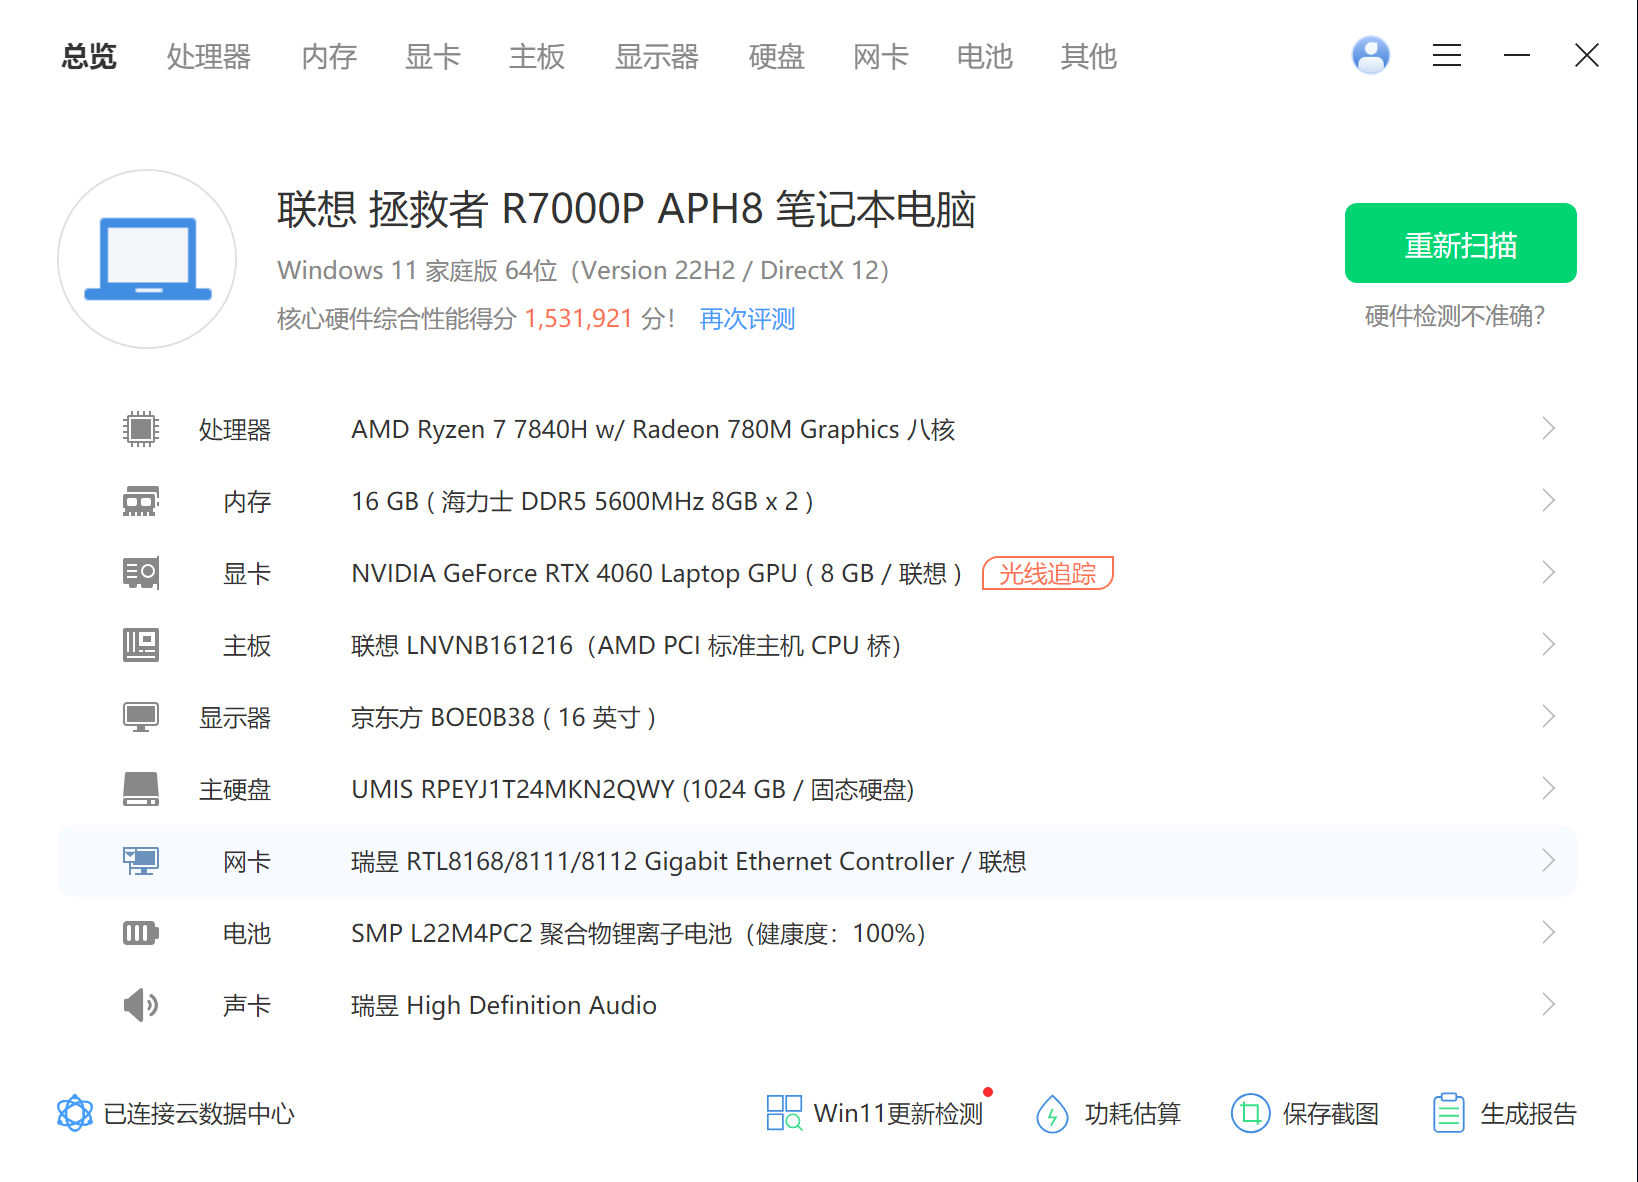
\includegraphics[width=0.7\linewidth]{3.png}
  \caption{sed进行数据替换}
   \end{figure}

\subsection{使用 awk 进行数据格式化}
我们可以使用 awk 来提取出时间戳和消息内容。例如,提取出日志的日期和消息内容:

\begin{verbatim}
 awk '{print $2, $3}' log.txt
  \end{verbatim}
结果将是:

\begin{figure}[H]
  \centering
    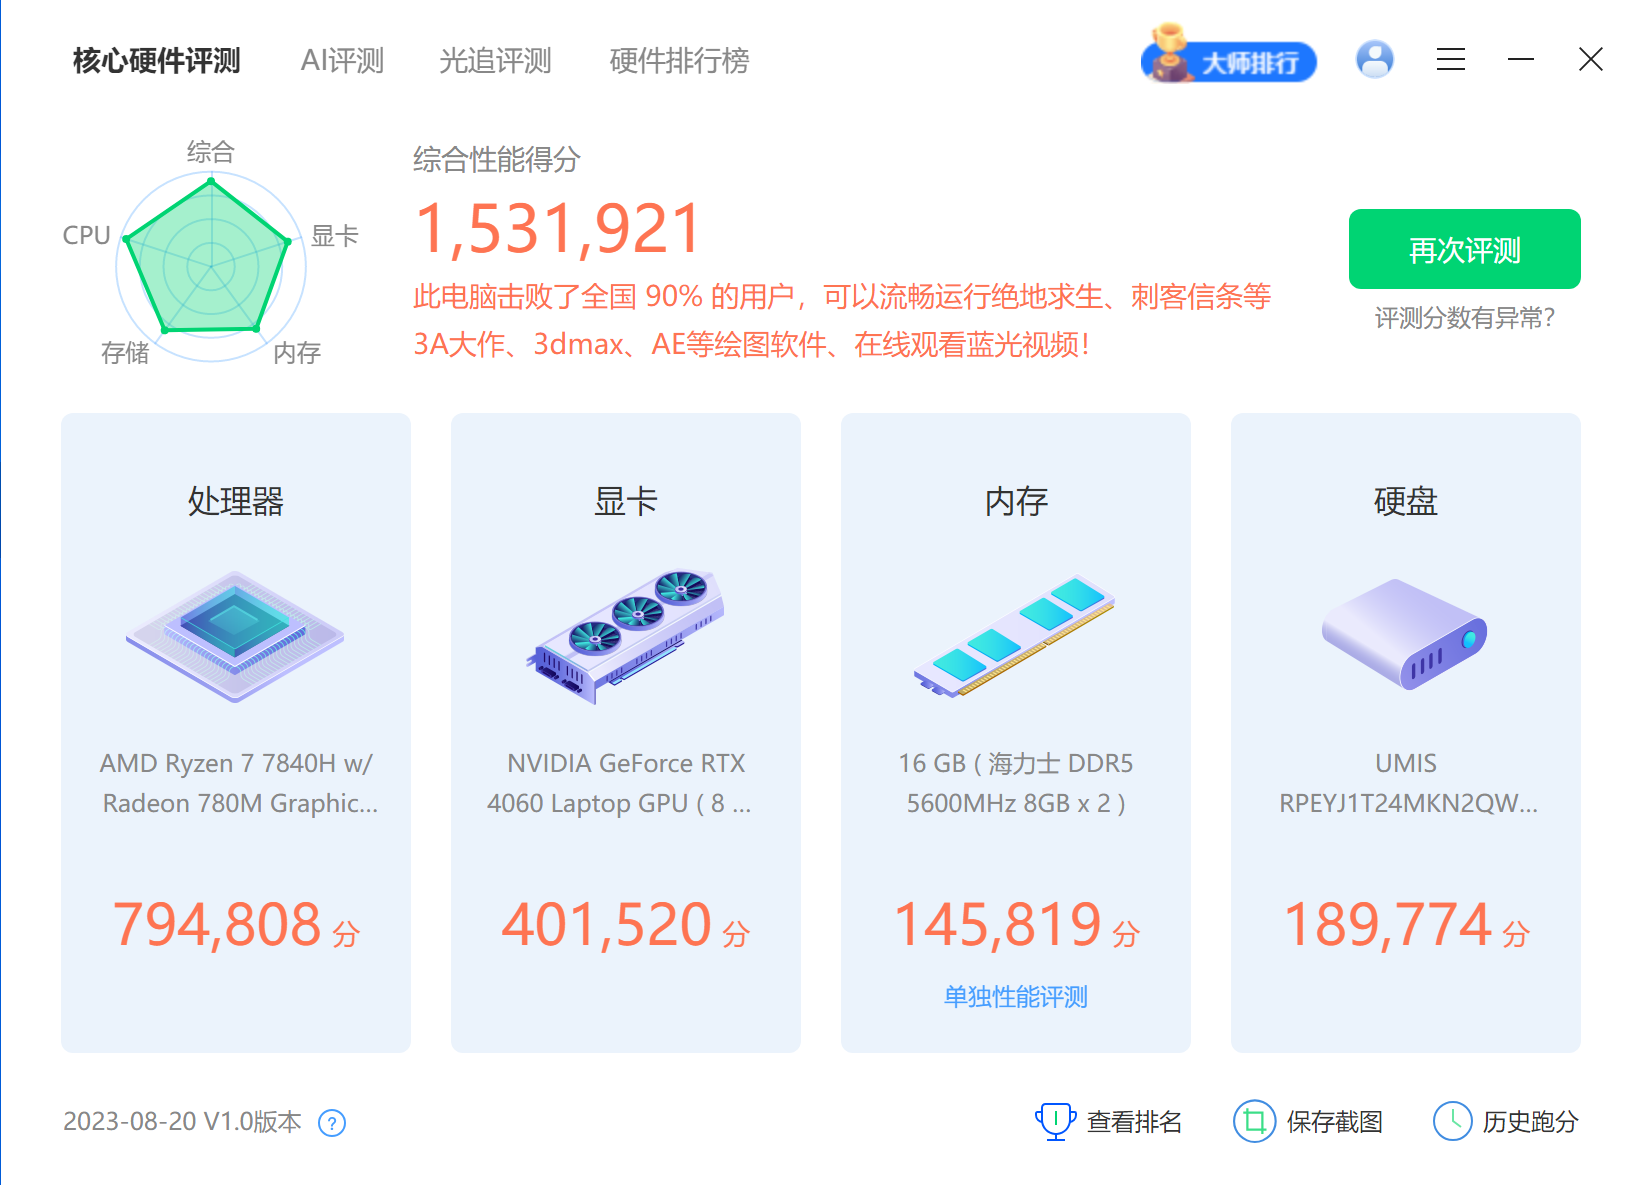
\includegraphics[width=0.7\linewidth]{4.png}
  \caption{数据格式化错误举例}
   \end{figure}
   
只输出了前半部分是因为 awk 按照空格分隔字段,日志中的某些消息有多个单词,如 "Connection established" 和 "Attempting to reconnect" 等。默认情况下,awk 将每个空格都视为一个字段分隔符,因此导致输出的是部分结果。
为了确保 awk 能正确提取完整的消息内容,可以将命令修改为只提取日期和从第三个字段开始的所有消息。可以使用 \$2 作为日期,\$3, \$4, \$5, ... 代表剩下的内容。一个更通用的方法是使用 \$2 后跟 \$0 的子串从第三个字段开始提取所有内容:

\begin{lstlisting}
awk '{print $2, substr($0, index($0,$3))}' log.txt
\end{lstlisting}

\begin{figure}[H]
  \centering
    \includegraphics[width=0.7\linewidth]{5.png}
  \caption{使用awk数据格式化}
   \end{figure}
   
   在这个命令中:\$2 提取第二个字段(日期)。
substr(\$0, index(\$0,\$3)) 提取从第三个字段到行末的内容,确保所有消息都被包含。

\begin{lstlisting}
2024-09-06 Connection established.
2024-09-06 Connection lost.
2024-09-06 Attempting to reconnect.
2024-09-06 Reconnection failed.
2024-09-06 Connection re-established.
\end{lstlisting}

\subsection{使用 sort 进行数据排序}
我们可以对日志进行排序,例如按时间顺序对日志条目进行排序:

\begin{figure}[H]
  \centering
    \includegraphics[width=0.7\linewidth]{6.png}
  \caption{log日志内容}
   \end{figure}
   
\begin{lstlisting}[language=bash]
sort -k2 log.txt
\end{lstlisting}

此命令将按照第二列(时间戳)进行排序。输出如下:

\begin{lstlisting}
ERROR 2024-09-06 Connection lost.
ERROR 2024-09-06 Reconnection failed.
INFO 2024-09-06 Attempting to reconnect.
INFO 2024-09-06 Connection established.
INFO 2024-09-06 Connection re-established.
\end{lstlisting}

\begin{figure}[H]
  \centering
    \includegraphics[width=0.7\linewidth]{7.png}
  \caption{使用sort对时间戳排序}
   \end{figure}

 如果日志有时间信息,你可以先按第二列(日期),再按第三列(实际的日志内容)进行排序。修改后的命令如下:
 
\begin{lstlisting}[language=bash]
sort -k2,2 -k3,3 log.txt
\end{lstlisting}

这个命令首先按日期排序(-k2,2),然后按消息的内容(-k3,3)排序,这样就能确保按时间顺序对条目进行排序,使日期相同。

\begin{figure}[H]
  \centering
    \includegraphics[width=0.7\linewidth]{8.png}
  \caption{有不同日期时间的日志}
   \end{figure}

\begin{figure}[H]
  \centering
    \includegraphics[width=0.7\linewidth]{9.png}
  \caption{排序结果}
   \end{figure}

\subsection{使用grep进行复杂日志处理}
 假设日志文件 log.txt 的结构变得更加复杂:
 \begin{figure}[H]
  \centering
    \includegraphics[width=0.7\linewidth]{10.png}
  \caption{复杂日志}
   \end{figure}

 筛选包含特定时间范围内的错误
假设你需要找出所有在 8:15 AM 到 8:30 AM 之间发生的错误。

\begin{verbatim}
 grep 'ERROR' log.txt | awk '$3 >= "08:15:00" && $3 <= "08:30:00"'
  \end{verbatim}

\begin{figure}[H]
  \centering
    \includegraphics[width=0.8\linewidth]{11.png}
  \caption{筛选结果}
   \end{figure}

\subsection{使用awk进行复杂日志处理}
 提取并统计特定服务器的错误数量
 
假设你想统计每个服务器发生错误的次数。

\begin{verbatim}
 grep 'ERROR' log.txt | awk -F'Source: ' '{print $2}' | awk '{print $1}' | sort | uniq -c
  \end{verbatim}

\begin{figure}[H]
  \centering
    \includegraphics[width=0.8\linewidth]{12.png}
  \caption{统计次数}
   \end{figure}

\subsection{使用awk进行平均值计算}
假设有一个文本文件 numbers.txt,其内容如下:
10
20
30
40
50
计算这些数字的总和和平均值:
\begin{verbatim}
awk '{sum+=$1} END {print "Sum:", sum, "Average:", sum/NR}' numbers.txt
  \end{verbatim}
  
\begin{figure}[H]
  \centering
    \includegraphics[width=0.8\linewidth]{13.png}
  \caption{平均值计算结果}
   \end{figure}

\subsection{文件内容比较和合并}
比较两个文件的差异
假设有两个文件 file1.txt 和 file2.txt,可以使用 diff 来查看差异:
diff file1.txt file2.txt
\begin{figure}[H]
  \centering
    \includegraphics[width=0.8\linewidth]{14.png}
  \caption{file1}
   \end{figure}
   
\begin{figure}[H]
  \centering
    \includegraphics[width=0.8\linewidth]{15.png}
  \caption{file2}
   \end{figure}


   \begin{figure}[H]
  \centering
    \includegraphics[width=0.8\linewidth]{16.png}
  \caption{file2}
   \end{figure}
   
  合并两个文件的内容
将 file1.txt 和 file2.txt 合并为一个文件 merge.txt:
cat file1.txt file2.txt > merged.txt
\begin{figure}[H]
  \centering
    \includegraphics[width=0.8\linewidth]{17.png}
  \caption{file2}
   \end{figure}

   \subsection{使用正则表达式}
假设有一个文本文件 file1.txt,其内容如下:
abc123
def456
ghi789
abc456
123abc
匹配以 abc 开头且以数字结尾的行:
\begin{verbatim}
grep '^abc.*[0-9]$' file1.txt
\end{verbatim}
  
\begin{figure}[H]
  \centering
    \includegraphics[width=0.8\linewidth]{29.png}
  \caption{匹配结果}
   \end{figure}
  
 \section{代码链接}
      请访问以下链接来查看我在Github上的相关练习、报告和代码:
\url{https://github.com/boken319/git_push}
我的在线Latex文件的网址:
\url{https://cn.overleaf.com/read/hkfqgccpxkdd#506bd5}

\end{document}
